\section{Introdução}

\begin{figure}[htb!]
  \centering
  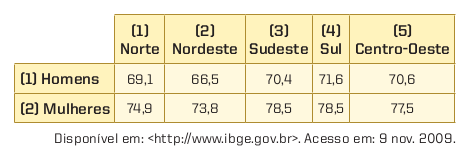
\includegraphics[width=.6\linewidth]{images/quadro.png}
  \caption{expectativa de vida brasileira em 2008}
  \label{fig:}
\end{figure}

Note que podemos encontrar a expectativa de vida de uma mulher residente na região Sul bastando olhar o cruzamento da linha 2 com a coluna 4, onde encontramos o valor de 78,5 anos. 

Em matemática, as tabelas como essa são chamadas de \textbf{matrizes}, sobre as quais definiremos a relação de igualdade e algumas operações. 

\section{Definição}
\dfn{Matriz}{Chama-se \textbf{matriz do tipo $m \times n$} (lemos ``m por n'') toda tabela de números dispostos em \textit{m} linhas e \textit{n} colunas.
} 

Essa tabela deve ser representada entre parênteses () ou entre colchetes [].

\begin{examples}\leavevmode

  \begin{tasks}
    \task{
      $\begin{bmatrix}
        -6 & 7 \\
        -4 & 0 \\
        2 & -1 \\
      \end{bmatrix}$ 
      é uma matriz do tipo $3 \times 2$, pois tem 3 linhas e 2 colunas.
    }
    \task {
    $\begin{bmatrix}
      3 & \sqrt{2} & -5
    \end{bmatrix}$
    é uma matriz do tipo $1 \times 3$, pois tem 1 linha e 3 colunas.
    }
  \end{tasks}
  
\end{examples}

\section{Representação genérica}

Indicamos por \textbf{$a_{ij}$} o elemento posicionado na linha \textit{i} e na coluna \textit{j} de uma matriz \textit{A}.

Na matriz:

\begin{equation*}
  A_{3 \times 2} = \begin{bmatrix}
    6 & 7 \\
    -4 & 0 \\
    2 & -1
  \end{bmatrix}
\end{equation*}

\begin{itemize}
  \item o elemento 6 está na linha 1 e na coluna 1; por isso, ele é indicado por $a_{11}$, ou seja, $a_{11} = 6$;
  \item o elemento 7 está na linha 1 e na coluna 2; por isso, ele é indicado por $a_{12}$, ou seja, $a_{12} = 7$;
  \item analogamente, temos $a_{21} = -4$, $a_{22} = 0$, $a_{31} = 2$, $a_{32} = -1$.
\end{itemize}

\dfn{Matriz Genérica}{
  Representamos genericamente uma matriz \textit{A} do tipo $m \times n$ da seguinte maneira:

  \begin{equation*}
    A_{m \times n} = \begin{bmatrix}
      a_{11} & a_{12} & a_{13} & \dots & a_{1n} \\
      a_{21} & a_{22} & a_{23} & \dots & a_{2n} \\
      \vdots & \vdots & \vdots & \vdots & \vdots \\
      a_{m1} & a_{m2} & a_{m3} & \dots & a_{mn} \\
    \end{bmatrix}
  \end{equation*}
}
  Como essa representação é muita extensa, vamos convencionar uma forma abreviada. Essa matriz pode ser representada simplesmente por 
  $A = (a_{ij})_{m \times n}$ ou, quando não houver possibilidade de confusão quanto ao tipo de matriz, por $A = (a_{ij})$.

\begin{exercise}
  Representar explicitamente a matriz $A = (a_{ij})_{2 \times 4}$ tal que $a_{ij} = 2i + j$.

  Primeiro, representamos genericamente a matriz \textit{A}, do tipo $2 \times 4$:
  \begin{equation*}
    A = \begin{bmatrix}
      a_{11} & a_{12} & a_{13} & a_{14} \\
      a_{21} & a_{22} & a_{23} & a_{24} \\
    \end{bmatrix}
  \end{equation*}

  A seguir, calculamos o valor de cada elemento $a_{ij}$, pela lei $a_{ij} = 2i + j$:

  \begin{tasks}(2)
    \task[] $a_{11} = 2 \cdot 1 + 1 = 3$
    \task[] $a_{12} = 2 \cdot 1 + 2 = 4$
    \task[] $a_{13} = 2 \cdot 1 + 3 = 5$
    \task[] $a_{14} = 2 \cdot 1 + 4 = 6$
    \task[] $a_{21} = 2 \cdot 2 + 1 = 5$
    \task[] $a_{22} = 2 \cdot 2 + 2 = 6$
    \task[] $a_{23} = 2 \cdot 2 + 3 = 7$
    \task[] $a_{24} = 2 \cdot 2 + 4 = 8$
  \end{tasks}

  Concluindo, temos a matriz: $A = \begin{bmatrix}
    3 & 4 & 5 & 6 \\
    5 & 6 & 7 & 8
  \end{bmatrix}$
\end{exercise}

\section{Matrizes Especiais}

\subsection{Matriz Quadrada}

\dfn{Matriz Quadrada}{É toda matriz cujo número de linhas é igual ao número de colunas.}

O número de linhas ou de colunas de uma matriz quadrada é chamado de \textbf{ordem} da matriz.

\begin{examples}\leavevmode
  \begin{tasks}(2)
    \task $\begin{bmatrix}
      4 & 9 & 0 \\
      -6 & 2 & 4 \\
      3 & 5 & -2
    \end{bmatrix}$
    é uma matriz quadrada de ordem 3.

    \task $\begin{bmatrix}
      3 & -9 \\
      0 & 1
    \end{bmatrix}$
    é uma matriz quadrada de ordem 2.
  \end{tasks}
\end{examples}

Numa matriz A de ordem \textit{n}, os elementos $a_{ij}$, tais que $i = j$ formam a \textbf{diagonal principal} da matriz, e os elementos 
$a_{ij}$, tais que $i + j = n + 1$ formam a \textbf{diagonal secundária}. Por exemplo:

\begin{figure}[htb!]
  \centering
  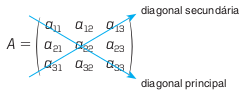
\includegraphics[width=.3\linewidth]{images/quadrada.png}
\end{figure}

\subsection{Matriz Identidade}

\dfn{Matriz Identidade}{É a matriz quadrada cujos elementos da \textbf{diagonal principal} são iguais a 1 e os demais iguais a 0.}

Indicamos por $I_n$ a matriz identidade de ordem \textit{n}.

\begin{examples}\leavevmode
  \begin{tasks}(2)
    \task $I_3 = \begin{bmatrix}
      1 & 0 & 0 \\
      0 & 1 & 0 \\
      0 & 0 & 1
    \end{bmatrix}$

    \task $I_2 = \begin{bmatrix}
      1 & 0 \\
      0 & 1
    \end{bmatrix}$
  \end{tasks}
\end{examples}

\subsection{Matriz Nula}

\dfn{Matriz Nula}{É a matriz que possui todos os elementos iguais a zero.}

\begin{examples}\leavevmode
  \begin{tasks}(2)
    \task 
  $\begin{bmatrix}
    0 & 0 & 0 \\
    0 & 0 & 0 \\
    0 & 0 & 0 \\
  \end{bmatrix}$
  \task $\begin{bmatrix}
    0 & 0 \\
    0 & 0 \\
  \end{bmatrix}$
  \end{tasks}
  
\end{examples}

\subsection{Transposta de uma Matriz}

\dfn{Transposta de uma Matriz}{Transposta de uma matriz \textit{A} é a matriz $A^t$ tal que os números que a formam são obtidos através da troca de posição entre linhas e colunas da matriz \textit{A}. }

\begin{examples}\leavevmode
  \begin{tasks}
    \task {A transposta de $A_{3 \times 2} = \begin{bmatrix}
        5 & -4 \\
        6 & 2 \\
        0 & 7
    \end{bmatrix}$
    é a matriz $A^t_{2 \times 3} = \begin{bmatrix}
      5 & 6 & 0 \\
      -4 & 2 & 7 \\
    \end{bmatrix}$
    }

    \task {A transposta de $B_{1 \times 4} = \begin{bmatrix}
        2 & 0 & -5 & 8 \\
    \end{bmatrix}$
    é a matriz $B^t_{4 \times 1} = \begin{bmatrix}
      2 \\
      0 \\
      -5 \\
      8
    \end{bmatrix}$
  }
  \end{tasks}
\end{examples}

Nome que a transposta de uma matriz $m \times n$ é uma matriz do tipo $n \times m$.

\subsection{Igualdade de Matrizes}
\dfn{Igualdade de Matrizes}{
  Duas Matrizes do mesmo tipo são iguais quando todos os elementos correspondentes são iguais.
}

\begin{exercise}
  Determinar o número real \textit{x} tal que: $\begin{bmatrix}
    6 & x^2-5 \\
    0 & x
  \end{bmatrix} = \begin{bmatrix}
    6 & 11 \\
    0 & 4
  \end{bmatrix}$

  \vspace{.3cm}
  \textbf{Resolução} \vspace{.3cm}

  As matrizes são do mesmo tipo $(2 \times 2)$. Logo, elas serão iguais se, e somente se, os elementos 
  correspondentes forem iguais, isto é:

  \begin{equation*}
    \begin{cases}
      6 = 6 \\
      x^2 - 5 = 11 \\
      0 = 0 \\
      x = 4
    \end{cases}
    \implies 
    \begin{cases}
      x^2 = 16 \\
      x = 4
    \end{cases}
    \therefore
    \begin{cases}
      x = \pm 4 \\
      x = 4
    \end{cases}
  \end{equation*}

  Como o número $4$ é a única solução comum às duas equações do sistema, concluímos que as matrizes são iguais se, e 
  somente se, $x = 4$.
  
\end{exercise}

\subsection{Exercícios Propostos}

\begin{enumerate}[label*=\protect\fbox{\arabic{enumi}}]
  \item {
      Uma rede comercial é formada por cinco lojas, numeradas de 1 a 5. A tabela abaixo mostra o faturamento, em real, de 
      cada loja nos quatro primeiros dias de janeiro:

      \begin{equation*}
          \begin{split}
            \begin{bmatrix}
              1950 & 2030 & 1800 & 1950 \\
              1500 & 1820 & 1740 & 1680 \\
              3010 & 2800 & 2700 & 3050 \\
              2500 & 2420 & 2300 & 2680 \\
              1800 & 2020 & 2040 & 1950 
            \end{bmatrix}
          \end{split}
      \end{equation*}

      Cada elemento $a_{ij}$ dessa matriz é o faturamento da loja \textit{i} no dia \textit{j}. 

      \begin{tasks}
        \task Qual foi o faturamento da loja 3 no dia 2?
        \task Qual foi o faturamento dessa rede de lojas no dia 3?
        \task Qual foi o faturamento da loja 1 nos quatro dias?
      \end{tasks}
    }
  \item {
      Represente explicitamente cada uma das matrizes:
      \begin{tasks}
        \task $A = (a_{ij})_{3 \times 2}$ tal que $a_{ij} = i + 2j$
        \task $B = (b_{ij})_{2 \times 3}$ tal que $b_{ij} = i^2 + 3j$
        \task $C = (c_{ij})_{2 \times 2}$ tal que $c_{ij} = 2i$
        \task $D = (a_{ij})_{2 \times 3}$ tal que $\begin{cases} 1, \text{ se } i = j \\ i + j, \text{ se } i \neq j \end{cases}$
      \end{tasks}
    }

  \item {
      Sendo $I_2$ a matriz identidade de ordem 2, determine o número real \textit{x} tal que:
      \begin{equation*}
          \begin{split}
            \begin{bmatrix}
              x^2 - 15 & 0 \\
              0 & x - 3 
            \end{bmatrix} = I_2
          \end{split}
      \end{equation*}
    }

  \item {
      Dada a matriz $A = \begin{bmatrix}
        5 & 4 & -2 \\
        -6 & 0 & 3
      \end{bmatrix}$,
      determine as matrizes:
      \begin{tasks}
        \task $A^t$
        \task $(A^t)^t$
      \end{tasks}
    }

  \item {
      Obtenha os valores reais de \textit{x} e \textit{y} de modo que a matriz abaixo seja nula.
      \begin{equation*}
          \begin{split}
            \begin{bmatrix}
              3x + y - 7 & 0 & 0 \\
              0 & 5x - y - 1 & 0
            \end{bmatrix}
          \end{split}
      \end{equation*}
    }
\end{enumerate}
  

\section{Operações entre Matrizes}

\subsection{Adição de matrizes}

\dfn{Adição de Matrizes}{
  A \textbf{soma} de duas matrizes do mesmo tipo, \textit{A} e \textit{B}, é a matriz em que cada elemento é a soma de seus 
  correspondentes em \textit{A} e \textit{B}. 

}

  Indicamos essa soma por: $A + B$.
\begin{example}
  \begin{equation*}
    \begin{bmatrix}
      4 & 7 \\
      -5 & 3 
    \end{bmatrix}
    + \begin{bmatrix}
      2 & 1 \\
      -3 & -6 
    \end{bmatrix}
    = \begin{bmatrix}
      6 & 8 \\
      -8 & -3 
    \end{bmatrix}
  \end{equation*}
\end{example}

\begin{proposition}{Adição de Matrizes}{trigsquare}
  \begin{enumerate}
    \item Associativa: $(A + B) + C = A + (B + C) = A + B + C$
    \item Comutativa: $A + B = B + A$
    \item Elemento Neutro: $A = 0 = 0 + A = A$. Onde $0$ é a \textbf{matriz nula}.
    \item Elemento oposto: $A + (-A) = (-A) + A = 0$. Onde $-A$ é a \textbf{matriz oposta} de \textit{A}.
  \end{enumerate}
\end{proposition}

\begin{example}
  Dado $A = \begin{bmatrix}
    2 & 0 \\
    7 & -8 
  \end{bmatrix}$,
  sua \textbf{matriz oposta} é $-A = \begin{bmatrix}
    -2 & 0 \\
    -7 & 8
  \end{bmatrix}$, pois:
  \begin{equation*}
    A + (-A) = \begin{bmatrix}
      2 & 0 \\
      7 & -8
    \end{bmatrix} + \begin{bmatrix}
      -2 & 0 \\
      -7 & 8 
    \end{bmatrix} = \begin{bmatrix}
      0 & 0 \\
      0 & 0
    \end{bmatrix}
  \end{equation*}
\end{example}

\subsection{Subtração de Matrizes}
\dfn{Subtração de Matrizes}{
  A \textbf{diferença} de duas matrizes do mesmo tipo, \textit{A} e \textit{B}, nessa ordem, é a soma de \textit{A} com 
  a oposta de \textit{B}.

}

  Indicamos essa diferença por $A - B$.
\begin{example}
  Sendo $A = \begin{bmatrix}
    9 & 6 \\
    4 & 0 \\
    -4 & -1
  \end{bmatrix}$ e $B = \begin{bmatrix}
    2 & 4 \\
    -3 & 5 \\
    1 & -1 \\
  \end{bmatrix}$, temos:
  
  \begin{equation*}
    A - B = A + (-B) = \begin{bmatrix}
      9 & 6 \\
      4 & 0 \\
      -4 & -1
    \end{bmatrix} + \begin{bmatrix}
      -2 & -4 \\
      3 & -5 \\
      -1 & 1
    \end{bmatrix} = \begin{bmatrix}
      7 & 2 \\
      7 & -5 \\
      -5 & 0
    \end{bmatrix} 
  \end{equation*}

  Para simplificar esse procedimento, podemos subtrair os elementos correspondentes em \textit{A} e \textit{B}:
  \begin{equation*}
    A - B = \begin{bmatrix}
      9 & 6 \\
      4 & 0 \\
      -4 & -1
    \end{bmatrix} - \begin{bmatrix}
      2 & 4 \\
      -3 & 5 \\
      1 & -1
    \end{bmatrix} = \begin{bmatrix}
      9 -2 & 6 - 4 \\
      4 - (-3) & 0 - 5 \\
      -4 -1 & -1 - (-1)
    \end{bmatrix} = \begin{bmatrix}
      7 & 2 \\
      7 & -5 \\
      -5 & 0
    \end{bmatrix}
  \end{equation*}
\end{example}

\subsection{Multiplicação de um número real por uma Matriz}

\dfn{Multiplicação de um número real por uma Matriz}{
  O \textbf{produto} de um número real \textit{k} por uma matriz \textit{A} é a matriz em que cada elemento é o 
  produto de seu correspondente em \textit{A} pelo número \textit{k}.

}

  Indicamos esse produto por $k \cdot A \text{ ou } kA $.
\begin{example}
  \[6 \cdot \begin{bmatrix}
    2 & 5 & 1 \\
    0 & \sqrt{2} & -2
  \end{bmatrix} = \begin{bmatrix}
    12 & 30 & 6 \\
    0 & 6\sqrt{2} & -12
  \end{bmatrix}\]
\end{example}

\subsection{Exercícios Propostos}

\begin{multicols}{2}
  \begin{enumerate}[label*=\protect\fbox{\arabic{enumi}}]
    \item {
      Dadas as matrizes $A = \begin{bmatrix}
        2 & 3 & 8 \\
        1 & -4 & 0
      \end{bmatrix}$, $B = \begin{bmatrix}
        4 & 5 & -9 \\
        6 & 2 & 7
      \end{bmatrix}$ e $C = \begin{bmatrix}
        2 & 0 \\
        8 & 6 \\
        -4 & 10
      \end{bmatrix}$ determine:
      \begin{tasks}
        \task $A + B$
        \task $2A - B$
        \task $3A - \frac{1}{2}\cdot C^t$
      \end{tasks}
    }

    \item {
        Determine a matriz \textit{X} tal que:
        \begin{equation*}
          2 \cdot \begin{bmatrix}
            4 & 1 & 3 \\
            6 & 2 & -1
          \end{bmatrix} + X = 3 \cdot \begin{bmatrix}
            1 & 2 & -1 \\
            0 & 2 & 1
          \end{bmatrix}
        \end{equation*}
      }

    \item {
        Determine as matrizes \textit{X} e \textit{Y} tais que: 
        \begin{equation*}
          X + Y = \begin{bmatrix}
            0 & 1 \\
            -6 & 4
          \end{bmatrix} \text{ e } X - Y = \begin{bmatrix}
            2 & -7 \\
            4 & 6
          \end{bmatrix} 
        \end{equation*} 
      }
  \end{enumerate}
\end{multicols}

\subsection{Multiplicação de Matrizes}

\dfn{Multiplicação de Matrizes}{
  O \textbf{produto} da matriz $A = (a_{ij})_{m \times n}$ pela matriz $B = (b_{ij})_{n \times p}$ é a matriz 
  $C = (c_{ij})_{m \times p}$ tal que cada elemento $c_{ij}$ é o produto da linha \textit{i} de \textit{A} pela coluna 
  \textit{j} de \textit{B}.
}

Esse produto é indicado por $A \cdot B$ ou $AB$.
O esquema a seguir ajuda a visualizar essa definição:

\vspace{.5cm}

% l' unite
\newcommand{\myunit}{1 cm}
\tikzset{
    node style sp/.style={draw,circle,minimum size=\myunit},
    node style ge/.style={circle,minimum size=\myunit},
    arrow style mul/.style={draw,sloped,midway,fill=white},
    arrow style plus/.style={midway,sloped,fill=white},
}

\begin{center}
  \begin{tikzpicture}[>=latex]
    % les matrices
    \matrix (A) [matrix of math nodes,
                nodes = {node style ge},
                 left delimiter  = (,
                 right delimiter = )] at (0,0)
    {
      a_{11} & a_{12} & \ldots & a_{1p}  \\
      |[node style sp]| a_{21}
             & |[node style sp]| a_{22}
                      & \ldots
                               & |[node style sp]| a_{2p} \\
      \vdots & \vdots & \ddots & \vdots  \\
      a_{n1} & a_{n2} & \ldots & a_{np}  \\
    };
    \node [draw,below=10pt] at (A.south) 
        { $A$ : \textcolor{red}{$n$ linhas} $p$ colunas};

    \matrix (B) [matrix of math nodes,
                 nodes = {node style ge},
                 left delimiter  = (,
                 right delimiter = )] at (6*\myunit,6*\myunit)
    {
      b_{11} & |[node style sp]| b_{12}
                      & \ldots & b_{1q}  \\
      b_{21} & |[node style sp]| b_{22}
                      & \ldots & b_{2q}  \\
      \vdots & \vdots & \ddots & \vdots  \\
      b_{p1} & |[node style sp]| b_{p2}
                      & \ldots & b_{pq}  \\
    };
    \node [draw,above=10pt] at (B.north) 
        { $B$ : $p$ linhas \textcolor{red}{$q$ colunas}};
    % matrice résultat
    \matrix (C) [matrix of math nodes,
                 nodes = {node style ge},
                 left delimiter  = (,
                 right delimiter = )] at (6*\myunit,0)
    {
      c_{11} & c_{12} & \ldots & c_{1q} \\
      c_{21} & |[node style sp,red]| c_{22}
                      & \ldots & c_{2q} \\
      \vdots & \vdots & \ddots & \vdots \\
      c_{n1} & c_{n2} & \ldots & c_{nq} \\
    };
    % les fleches
    \draw[blue] (A-2-1.north) -- (C-2-2.north);
    \draw[blue] (A-2-1.south) -- (C-2-2.south);
    \draw[blue] (B-1-2.west)  -- (C-2-2.west);
    \draw[blue] (B-1-2.east)  -- (C-2-2.east);
    \draw[<->,red](A-2-1) to[in=180,out=90]
      node[arrow style mul] (x) {$a_{21}\times b_{12}$} (B-1-2);
    \draw[<->,red](A-2-2) to[in=180,out=90]
      node[arrow style mul] (y) {$a_{22}\times b_{22}$} (B-2-2);
    \draw[<->,red](A-2-4) to[in=180,out=90]
      node[arrow style mul] (z) {$a_{2p}\times b_{p2}$} (B-4-2);
    \draw[red,->] (x) to node[arrow style plus] {$+$} (y)%
        to node[arrow style plus] {$+\raisebox{.5ex}{\ldots}+$} (z)
        to (C-2-2.north west);


    \node [draw,below=10pt] at (C.south) 
        {$ C=A\times B$ : \textcolor{red}{$n$ linhas}
                          \textcolor{red}{$q$ colunas}};

  \end{tikzpicture}
\end{center}

\begin{examples}\leavevmode
  \begin{enumerate}
    \item {
        $\begin{bmatrix}
          2 & 1 & 3 
        \end{bmatrix} \cdot \begin{bmatrix}
          5 & 3 \\
          2 & 0 \\
          1 & -2
        \end{bmatrix} = \begin{bmatrix}
          2 \cdot 5 + 1 \cdot 2 + 3 \cdot 1 & 2 \cdot 3 + 1 \cdot 0 + 3 \cdot (-2)
        \end{bmatrix} = \begin{bmatrix}
          15 & 0
        \end{bmatrix}$
      }

    \item {
        $\begin{bmatrix}
          3 & 5 \\ 
          2 & 0 
        \end{bmatrix} \cdot  \begin{bmatrix}
          4 & 5 & -2 \\
          2 & 1 & 3
        \end{bmatrix} = \begin{bmatrix}
          3 \cdot 4 + 5 \cdot 2 & 3 \cdot 5 + 5 \cdot 1 & 3 \cdot (-2) + 5 \cdot 3 \\
          2 \cdot 4 + 0 \cdot 2 & 2 \cdot 5 + 0 \cdot 1 & 2 \cdot (-2) + 0 \cdot 3
        \end{bmatrix} = \begin{bmatrix}
          22 & 20 & 9 \\
          8 & 10 & -4
        \end{bmatrix}$
      }
  \end{enumerate}
\end{examples}

\begin{note}
  \begin{enumerate}
    \item Se \textit{A} e \textit{B} são matrizes, existe o produto $AB$ se, e somente se, o número de colunas 
      de \textit{A} é igual ao número de linhas de \textit{B}. Veja abaixo:
      \begin{tasks}(2)
        \task {
          Existe o produto $A_{3 \times 4} \cdot B_{4 \times 5}$
        }
        \task Não existe o produto $A_{2 \times 3} \cdot B_{4 \times 2}$
      \end{tasks}
    \item {
        A matriz \textit{C}, tal que $C = AB$, possui o mesmo número de linhas de \textit{A} e o mesmo número de colunas 
        de \textit{B}, isto é:
        \begin{equation*}
          A_{m \times k} \cdot B_{k \times n} = C_{m \times n}
        \end{equation*}

        Por exemplo:
        
        \begin{tasks}(2)
          \task $A_{3 \times 5} \cdot B_{5 \times 8} = C_{3 \times 8}$
          \task $A_{1 \times 4} \cdot B_{4 \times 1} = C_{1 \times 1}$ 
        \end{tasks}
      }
  \end{enumerate}
\end{note}

\begin{proposition}{Propriedades da multiplicação de matrizes}{}
  \begin{enumerate}
    \item Associativa: $(A \cdot B) \cdot C = A \cdot (B \cdot C) = A \cdot B \cdot C$, em que $A_{m \times n}$, $B_{n \times k}$ e $C_{k \times p}$.
    \item Distributiva: $(A + B) \cdot C = A \cdot C + B \cdot C$, em que $A_{m \times n}$, $B_{m \times n}$ e $C_{k \times m}$.
    \item Elemento neutro: $A \cdot I_n = A$ e $I_m \cdot A = A$
    \item Transposta do produto: $(A \cdot B)^t = B^t \cdot A^t$, em que $A_{m \times n}$ e $B_{n \times k}$.
  \end{enumerate}
\end{proposition}

\begin{exercise}\leavevmode
  \begin{enumerate}
    \item {
        Determinar a matriz \textit{X} tal que: $\begin{bmatrix}
          2 & 3 \\
          1 & -4
        \end{bmatrix} \cdot X = \begin{bmatrix}
          4 \\
          -9
        \end{bmatrix}$

        \vspace{.3cm}
        \textbf{Resolução}
        \vspace{.3cm}

        Primeiro, vamos determinar o tipo da matriz \textit{X}:

        \begin{equation*}
          \begin{bmatrix}
            2 & 3 \\
            1 & -4 
          \end{bmatrix}_{2 \times 2} \cdot X_{m \times n} = \begin{bmatrix}
            4 & -9
          \end{bmatrix}_{2 \times 1}
        \end{equation*}

        Para que seja possível multiplicar as matrizes, o número de colunas da primeira
        matriz deve ser igual ao número de linhas de \textit{X}; portanto, $m = 2$. O número 
        de colunas da matriz \textit{X} deve ser igual ao número de colunas da matriz produto; 
        portanto, $n = 1$.

        Assim, a matriz \textit{X} é to tipo $2 \times 1$.

        Sendo $X = \begin{bmatrix}
          a \\ b
        \end{bmatrix}$, temos:

        \begin{equation*}
          \begin{bmatrix}
            2 & 3 \\
            1 & -4
          \end{bmatrix} \cdot \begin{bmatrix}
            a \\
            b
          \end{bmatrix} = \begin{bmatrix}
            4 \\
            -9
          \end{bmatrix} \implies \begin{bmatrix}
            2a + 3b \\
            a - 4b
          \end{bmatrix} = \begin{bmatrix}
            4 \\
            -9
          \end{bmatrix}
        \end{equation*}

        Portanto: \[
          \systeme{
            2a + 3b = 4,
            a - 4b = -9
          } \implies 
          \systeme{
            2a + 3b = 4,
            -2a + 8b = 18
          } \implies  
          0a + 11b = 22 \implies b = 2 \implies a = -1 
        \]

        Assim, concluímos: $X = \begin{bmatrix}
          -1 \\
          2
        \end{bmatrix}$
      }
  \end{enumerate}
\end{exercise}

\subsection{Exercícios Propostos}

\begin{enumerate}[label*=\protect\fbox{\arabic{enumi}}]
  \item{ Dadas as matrizes $A = \begin{bmatrix}
    2 & 6 \\
    -1 & 0 
  \end{bmatrix}$, $B = \begin{bmatrix}
    4 \\
    3
  \end{bmatrix}$ e $C = \begin{bmatrix}
    1 & -2
  \end{bmatrix}$, determine, se possível:

  \begin{tasks}(3)
    \task $A \cdot B$
    \task $A \cdot C$
    \task $B \cdot C$
    \task $A^2$
    \task $B^2$
  \end{tasks}
}
\item {
    Sendo as matrizes $A = \begin{bmatrix}
      1 & 2 & 3 \\
      0 & 6 & 1
    \end{bmatrix}$, $B = \begin{bmatrix}
      1 & 1 \\
      4 & 4 \\
      2 & 2 
    \end{bmatrix}$ e $C = \begin{bmatrix}
      1 & -1 & 1 \\
      -1 & 1 & -1
    \end{bmatrix}$, determine:

    \begin{tasks}(3)
      \task $A \cdot B$
      \task $B \cdot A$
      \task $A \cdot I_3$
      \task $I_2 \cdot A$
      \task $B \cdot C$
    \end{tasks}
  }

  \item{
      O valor de \textit{a} para que a setença $\begin{bmatrix}
        2 & 1 \\
        1 & 1
      \end{bmatrix} \cdot  \begin{bmatrix}
        1 & -1 \\
        -1 & a
      \end{bmatrix} = \begin{bmatrix}
        1 & 0 \\
        0 & 1
      \end{bmatrix}$ seja verdadeira é:

      \begin{tasks}(3)
        \task 1
        \task 2
        \task 0
        \task -2
        \task -1
      \end{tasks}
    }

  \item {
      Dadas as matrizes $A = (a_{ij})_{9 \times 8}$, com $a_{ij} = 2j$; $B = (b_{ij})_{8 \times 6}$, com $b_{ij} = i$; e $C \cdot A$,
      determine o elemento $C_{45}$ da matriz \textit{C}.
    }

  \item {
      Dadas as matrizes $A = \begin{bmatrix}
        1 & 2\\
        0 & -3
      \end{bmatrix}$, $B = \begin{bmatrix}
        6 \\
        -15
      \end{bmatrix}$, obtenha a matriz \textit{X} tal que $A \cdot X = B$.
    }
\end{enumerate}

\subsection{Matrizes Inversas}

\dfn{Matrizes Inversas}{
  Uma matriz \textit{A} de ordem \textit{n} é \textbf{invertível} se, e somente se, 
  existe uma matriz \textit{B} tal que:
  \begin{equation*}
    AB = BA = I_n
  \end{equation*}
  em que $I_n$ é a matriz identidade de ordem \textit{n}.
}

\begin{example}
  As matrizes $A = \begin{bmatrix}
    1 & 1 \\
    3 & 4
  \end{bmatrix}$ e $B = \begin{bmatrix}
    4 & -1\\
    -3 & 1
  \end{bmatrix}$ são inversas entre si, pois:
  \begin{equation*}
    AB = \begin{bmatrix}
      1 & 1 \\
      3 & 4
    \end{bmatrix} \cdot \begin{bmatrix}
      4 & -1 \\
      -3 & 1
    \end{bmatrix} = \begin{bmatrix}
      1 & 0 \\
      0 & 1 \\
    \end{bmatrix} = I_2 \text{  e  } BA = \begin{bmatrix}
      4 & -1 \\
      -3 & 1
    \end{bmatrix} \cdot \begin{bmatrix}
      1 & 1 \\
      3 & 4
    \end{bmatrix} = \begin{bmatrix}
      1 & 0 \\
      0 & 1
    \end{bmatrix} = I_2
  \end{equation*} 
  Assim, indicamos $B = A^{-1}$ ou, de maneira equivalente, $A = B^{-1}$.
\end{example}

\begin{exercise}\leavevmode
  Determinar, se existir, a inversa de cada uma das matrizes.

  \begin{tasks}(2)
    \task $A = \begin{bmatrix}
      1 & 3 \\
      0 & 2
    \end{bmatrix}$

    \task $B = \begin{bmatrix}
      1 & 2 \\
      2 & 4
    \end{bmatrix}$
  \end{tasks}

  \vspace{.3cm}
  \textbf{Resolução} \vspace{.3cm}

  \begin{tasks}
    \task {
      Admitindo que $A^{-1} = \begin{bmatrix}
        a & b \\
        c & d
      \end{bmatrix}$ seja a inversa da matriz \textit{A}, devemos ter 
      $A \cdot A^{-1} = I_2$, ou seja:
      \begin{equation*}
        \begin{bmatrix}
          1 & 3 \\
          0 & 2
        \end{bmatrix} \cdot \begin{bmatrix}
          a & b \\
          c & d
        \end{bmatrix} = \begin{bmatrix}
          1 & 0 \\
          0 & 1
        \end{bmatrix} \implies \begin{bmatrix}
          a+3c & b+3d \\
          2c & 2d
        \end{bmatrix} = \begin{bmatrix}
          1 & 0 \\
          0 & 1
        \end{bmatrix}
      \end{equation*}
      Igualando as matrizes, encontramos:
      \systeme{
        a + 3c = 1,
        2c = 0,
        b + 3d = 0,
        2d = 1
      } $\implies $ 
      \systeme{
        a + 3c = 1@(1),
        c = 0@(2),
        b+3d = 0@(3),
        d=\frac{1}{2}@(4)
      }

      Substituindo (2) em (1), obtemos: $a = 1$

      Substituindo (4) em (3), obtemos: $b = -\frac{3}{2}$

      Assim, concluímos: $A^{-1} = \begin{bmatrix}
        1 & -\frac{3}{2} \\
        0 & \frac{1}{2}
      \end{bmatrix}$
    }

    \task {
      Admitindo que $B^{-1} = \begin{bmatrix}
        a & b \\
        c & d
      \end{bmatrix}$ seja a inversa da matriz \textit{B}, devemos ter 
      $B \cdot B^{-1} = I_2$, ou seja:
      \begin{equation*}
        \begin{bmatrix}
          1 & 2 \\
          2 & 4
        \end{bmatrix} \cdot \begin{bmatrix}
          a & b \\
          c & d
        \end{bmatrix} = \begin{bmatrix}
          1 & 0 \\
          0 & 1
        \end{bmatrix} \implies \begin{bmatrix}
          a+2c & b+2d \\
          2a+4c & 2b+4d
        \end{bmatrix} = \begin{bmatrix}
          1 & 0 \\
          0 & 1
        \end{bmatrix}
      \end{equation*}

      Igualando as matrizes, encontramos:
      \systeme{
        a+2c = 1,
        2a+4c = 0,
        b+2d = 0,
        2b+4d=1
      } $\implies $
      \systeme{
        a+2c = 1@(1),
        a+2c=0@(2),
        b+2d=0@(3),
        b+2d=\frac{1}{2}@(4)
      }

      Logo, o sistema é impossível de responder, pois não existe solução e dessa forma 
      não existe matriz inversa de \textit{B}.
    }
  \end{tasks}
\end{exercise}

\subsection{Exercícios Propostos}

\begin{enumerate}[label*=\protect\fbox{\arabic{enumi}}]
  \item {
      Obtenha, se existir, a inversa de cada matriz:
      \begin{tasks}(4)
        \task $A = \begin{bmatrix}
          3 & 6 \\
          0 & 1
        \end{bmatrix}$
        \task $B = \begin{bmatrix}
          3 & 5 \\
          1 & 2 
        \end{bmatrix}$
        \task $C = \begin{bmatrix}
          1 & 1 \\
          1 & 1
        \end{bmatrix}$
        \task $D = \begin{bmatrix}
          0 & 2 & 0 \\
          0 & 0 & 1 \\
          1 & 0 & 0
        \end{bmatrix}$
      \end{tasks}
    }
    
\end{enumerate}
